\documentclass[12pt]{article}
\usepackage{amsgen,amsmath,amstext,amsbsy,amsopn,amssymb}
%\usepackage[dvips]{graphicx,color}
\usepackage{graphicx,color}
\usepackage{graphicx,color,bm}
\usepackage{epsfig}
\usepackage{enumerate}
\usepackage{float}
\usepackage{multicol}
\usepackage{longtable}
\usepackage{verbatim}
\usepackage{hyperref}
\usepackage[utf8]{inputenc}
\usepackage[english]{babel}
\usepackage{wrapfig,lipsum,booktabs}
\usepackage{commath}
\usepackage{wrapfig,lipsum,booktabs}
%\setlength{\oddsidemargin}{0.1 in} \setlength{\evensidemargin}{-0.1
%in} \setlength{\topmargin}{-0.6 in} \setlength{\textwidth}{6.5 in}
%\setlength{\textheight}{8.5 in} \setlength{\headsep}{0.75 in}
%\setlength{\parindent}{0 in} \setlength{\parskip}{0.1 in}

\textwidth 6.3in \textheight 8.8in \topmargin -0.5truein
\oddsidemargin .15truein
\parskip .1in
\renewcommand{\baselinestretch}{1.00}  % double spaced
\renewcommand{\thesection}{\Roman{section}} 
\renewcommand{\thesubsection}{\thesection.\Roman{subsection}}
\newcommand*{\addheight}[2][.5ex]{%
	\raisebox{0pt}[\dimexpr\height+(#1)\relax]{#2}%
}
\usepackage{caption}

\begin{document}
	
	\title{Homework 1, CSE 515}
	\author{\bf Alexander Van Roijen}
	
	\maketitle
	
	\section{2.1} As an if and only if proof, we seek to prove each direction given either side as truth and showing the latter. 
	\\
	\\
	Lets start with ($\rightarrow$). More explicitly, we have $P(x,y|z) = P(x|z)*P(y|z)$ by the defintion of conditional independence. We want to show that $P(x,y,z) = h(x,z)g(y,z)$
	
	\begin{gather}
		P(x,y|z) = P(x|z)*P(y|z) => \\
		\frac{P(x,y,z)}{P(z)} = \frac{P(x,z)}{P(z)}\frac{P(y,z)}{P(z)} => \\
		P(x,y,z) = \frac{P(x,z)}{P(z)}\frac{P(y,z)}{P(z)}P(z) => \\
		P(x,y,z) = h(x,z)g(y,z) 
	\end{gather}
	The last step is rather intuitive as all we have done is define $h(x,z) = \frac{P(x,z)}{P(z)}$ and $g(y,z) = P(y|z)$
	
	($\leftarrow$) Now we have that $P(x,y,z) = h(x,z)g(y,z)$ and want to show $P(x,y|z) = P(x|z)*P(y|z)$
	\begin{gather}
		\Sigma_{x} P(x,y,z) = P(y,z) = \Sigma_{x} h(x,z)g(y,z) = g(y,z)\Sigma_{x} h(x,z) \\
		\Sigma_{y} P(x,y,z) = P(x,z) = \Sigma_{y} h(x,z)g(y,z) = h(x,z)\Sigma_{y} g(y,z)\\
		\Sigma_{x}\Sigma_{y}  P(x,y,z) = P(z) = \Sigma_{x} \Sigma_{y} h(x,z)g(y,z) = \Sigma_{x}h(x,z)\Sigma_{y} g(y,z)\\
		\rightarrow P(x,y|z) = \frac{P(x,y,z)}{P(z)} \\
		\rightarrow P(x,y|z) = \frac{h(x,z)g(y,z)}{\Sigma_{x}h(x,z)\Sigma_{y} g(y,z)} \\
		 P(x|z) = \frac{P(x,z)}{P(z)} = \frac{h(x,z)\Sigma_{y} g(y,z)}{\Sigma_{x}h(x,z)\Sigma_{y} g(y,z)} = \frac{h(x,z)}{\Sigma_{x}h(x,z)} \\
		 P(y|z) = \frac{P(y,z)}{P(z)} = \frac{g(y,z)\Sigma_{x} h(x,z)}{\Sigma_{x}h(x,z)\Sigma_{y} g(y,z)} = \frac{g(y,z)}{\Sigma_{y} g(y,z)} \\
		 \rightarrow  P(x,y|z) = P(x|z)P(y|z) = \frac{h(x,z)g(y,z)}{\Sigma_{x}h(x,z)\Sigma_{y} g(y,z)}\\
		  \square
	\end{gather}
	$ \Sigma_{x} P(x,y,z) = P(y,z) = \Sigma_{x} h(x,z)g(y,z)$
	$P(x,y,z)=P(x,y|z)P(z) = h(x,z)g(y,z) => P(x,y|z) = \frac{h(x,z)g(y,z)}{P(z)}$
	
	\section{2.2} 
	\subsection{a}
	We want to show that simply swapping our random variables such that $x_1 \leftrightarrow x_4$ and $x_2 \leftrightarrow x_3$ we still get $P(x_1,x_2,x_3,x_4) = P(x_4,x_3,x_2,x_1)$
	\\
	This is easily seen by simple flipping bits from our original table to get the following 
	\begin{table}[H]
		\begin{center}
			\begin{tabular}{ c c c c }
				\hline

				(0,0,0,0)&(0,0,0,1)&(0,0,1,1)&(0,1,1,1)\\
				(1,0,0,0)&(1,1,0,0)&(1,1,1,0)&(1,1,1,1)\\
				\hline
			\end{tabular}
			\caption{We get the same set of possible configurations with the same density}
		\end{center}
	\end{table}
	\subsection{b}
	We have 4 possibilities\\
	\begin{itemize}
		\item $x_2=0,x_4=0$ We are left with these states (1,0,0,0) (0,0,0,0). We know for a fact that $x_3 = 0$
		\item $x_2=0,x_4=1$ We are left with these states (0,0,0,1) (0,0,1,1). We know for a fact that $x_1 = 0$  
		\item $x_2=1,x_4=0$ We are left with these states (1,1,0,0) (1,1,1,0). We know for a fact that $x_1 = 1$  
		\item $x_2=1,x_4=1$ We are left with these states (1,1,1,1) (0,1,1,1). We know for a fact that $x_3 = 1$  
	\end{itemize}
This shows conditional independence as no matter what we know about $x_1$ and $x_3$, it wont reveal anything we wouldnt already know about the other.
	\subsection{c}
	Prove by contradiction, we will show that $P(x_1,x_2,x_3,x_4)$ cannot be factorized according to the hammersley-clifford Theorem, or in particular\\
	$P(x_1,x_2,x_3,x_4) = g(x_1,x_2)h(x_2,x_3)j(x_3,x_4)k(x_4,x_1)$
	We have 
	\begin{gather}
	P(0,0,0,0) = \frac{1}{8} = g(0,0)h(0,0)j(0,0)k(0,0)\\
	P(0,0,1,0) = 0 = g(0,0)h(0,1)j(1,0)k(0,0)\\
	P(0,0,1,1) = \frac{1}{8} = g(0,0)h(0,1)j(1,1)k(1,0)\\
	P(1,1,1,0) = \frac{1}{8} = g(1,1)h(1,1)j(1,0)k(0,1)
	\end{gather}
	Accordingly, we know that one of $g(0,0)h(0,1)j(1,0)k(0,0)$ must be zero.\\
	However,
	\\
	If $g(0,0)$ was 0, then that would contradict 5 and 7. 
	\\
	If $h(0,1)$ was 0, then that would contradict 7
	\\
	If $j(1,0)$ was 0, that would contradict 8
	\\
	Finally if $k(0,0)$ was 0, that would contradict 5.
	
	Contradiction! We cant satisfy this set of requirements, thus our assumption that $P(x_1,x_2,x_3,x_4) = g(x_1,x_2)h(x_2,x_3)j(x_3,x_4)k(x_4,x_1)$ is wrong. $\square$

\section{2.3}
\subsection{a}
$P_{IS(G)}(S) = \frac{1}{\vert Z \vert}I(S\in IS(G))$
We have that the only time the above function is equal to one only when a subset S, represented by a vector x, is in $IS(G)$. Equivalently, if $(i,j)\in E \rightarrow (i,j) \notin S$ so $P_{IS(G)}(S) = \frac{1}{\vert Z \vert}\Pi_{i,j\in E}f(i,j)$
\\
Accordingly $P_G(X)$ where $x$ is ${0,1}$ of size $\lvert V \lvert$, we can represent its probability in this manner as $\frac{1}{\vert Z \vert}\Pi_{i,j\in E}(1-I(xi=xj=1))$ as we know that if any two edges connect when both $x_i,x_j$ are present,we have found an edge that makes our $S$ no longer an independent subset and should have probability zero.

\subsection{b}

You can imagine this graph as simple ordered pairs, as in $x_1$ connects to $x_2, x_2$ to $x_3$, and so on. In the simplest of cases, $Z(l_n) = 2,3,5$ when n = 1,2,3 respectively. We get 
$\begin{bmatrix}
	Z(l_n) \\
	Z(l_{n-1})
\end{bmatrix}$ = 
$\begin{bmatrix}
1&1 \\
1&0
\end{bmatrix}$
$\begin{bmatrix}
Z(l_{n-1}) \\
Z(l_{n-2})
\end{bmatrix}$
\\
\\
So, to solve it we want 
$\begin{bmatrix}
Z(l_n) \\
Z(l_{n-1})
\end{bmatrix}$ = 
$\begin{bmatrix}
1&1 \\
1&0
\end{bmatrix}$$^{(n-1)}$
$\begin{bmatrix}
3 \\
2
\end{bmatrix}$
by substituting in the values for $Z(l_1) \& Z(l_2)$ However, to solve for $\begin{bmatrix}
1&1 \\
1&0
\end{bmatrix}$$^{(n-1)}$ we will need to diagonalize it. lets call $\begin{bmatrix}
1&1 \\
1&0
\end{bmatrix}$ A instead, so we are trying to diagonalize A.

$det(A-I\lambda) = $det($\begin{bmatrix}
1-\lambda&1 \\
1&-\lambda
\end{bmatrix}$) = $-\lambda(1-\lambda) - 1 = \lambda^2 - \lambda -1$
\\
$\lambda^2 - \lambda -1 = 0 \rightarrow \lambda^2 - \lambda = 1$
\\
Our eigen values are thus $\lambda_1 = \frac{1-\sqrt{5}}{2}$ and $\lambda_2= \frac{1+\sqrt{5}}{2}$ \\
After this comes a larger proof, some additional details and reference can be found in the appendix.
\\
\\
Solving all this gives us $Fib(n) = \frac{1}{\sqrt5}((\frac{1+\sqrt5}{2})^{n+1} - (\frac{1-\sqrt5}{2})^{n+1}) = Z(l_n)$



\subsection{c}

We can intuitively see that for any $i \in S \rightarrow i=1$, it inherently means that \\
$i-1 = 0 \& i+1 = 0$. The remainder of the nodes are free to have their own number of permutations, which is exactly $Z_{left} = fib(left)$ and $Z_{right} = fib(right)$. What are the sizes of the left and right side? They are exactly $i-2$ and $n-i-1$ unless we are at the very edges, where $i=n$ or $i=1$ which results in $Z_{left}=1$ and $Z_{right} = fib(n-2)$ and vice versa. Which leaves us with the general rule 
$P_{Ln}(i)=\frac{Z_{left}Z_{right}}{Z_{L_n}} = \frac{Z_{i-2}Z_{n-i-1}}{Z_{n}} = \frac{Fib_{i-2}Fib_{n-i-1}}{Fib_{n}}$.A fun exercise could be to plug in the closed form solution and simplify, but that is an exercise for another time.\\
 The graphic below highlights the distribution of our $P$ over a chain of 11 nodes.
\begin{figure}[H]
	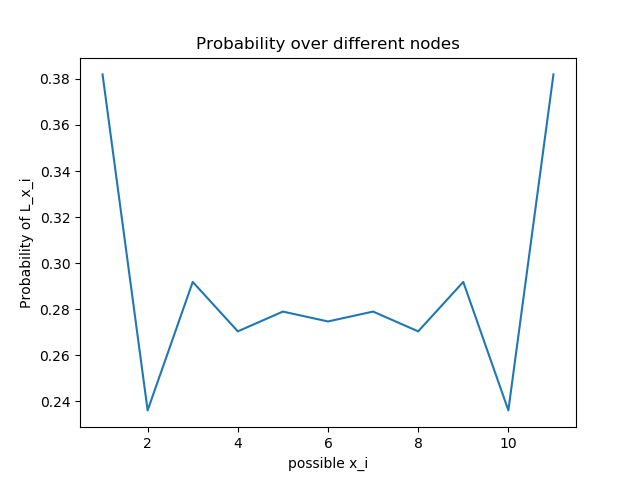
\includegraphics[width=0.5\textwidth]{p2_3.png}
	\caption{$P_{Ln}(i)$ over $i = 1...11$}
\end{figure}

Looking at this graph and the probabilities we derived before, the graph makes intuitive sense. It should be symmetric, and it is, around the center node of our chain, as we have similar numbers of nodes on each side and thus have similar independent set sizes. Furthermore, the highest probabilities are at the very edge as we only limit the number of fixed node values by one whole node, meanwhile at the second node, we lose one whole node without any gain, before finally moving to the third where we get one node on our left side back. Looking at our equation might also be fruitful, d imagine that by playing around with multiplying two fibonacci numbers together versus adding their respective values $n$ and then getting that fibonnaci number might highlight the kind of relationship that we are seeing here, most likely being somewhere in the realm of $fib(n_1+n_2) \ge fib(n_1)*fib(n_2)$ perhaps.
\subsection{d}
$P_{Ln}(x) = P(x_1)*P(x_2|x_1)*...P(x_n|x_{n-1}..x_1)$ Knowing the independencies we get $P_{Ln}(x) = P(x_1)*P(x_2|x_1)*...P(x_n|x_{n-1})$ This is intuitive both from the graph that mimics this Bayesian network and the chain rule. Now what this means is that the probability of any particular set S represented by a vector X is some multiple of the rules we developed before, all we need to do is discover what that general rule is.
\\
Its easy to see that $P(x_1) = \frac{fib(n-2)}{fib(n)}$. Note that this denominator will be present for the remainder of our conditional probabilities, but wont be explicitly noted.
\\
For each subsequent set of $x_i$ we have that we know $x_{i-1}$ and $x_i$ are known, meaning according to our previous recursion we get $\frac{P(x_{i-1},x_i)}{P(x_{i-1})} = \frac{Fib_{i-2}Fib_{n-i-1 }}{Fib_{n}} $

\section{2.4}
\subsection{a}

we have $|Z_{l}| = |Z_{l}(0)| + |Z_{l}(1)|$ and $|Z_l(0)| = \Sigma_{k=1}^n \binom{n}{k} |Z_{l-1}(1)|^{k}|Z_{l-1}(0)|^{n-k} = (|Z_{l-1}(0)| + |Z_{l-1}(1)|)^k$ and $|Z_l(1)| = |Z_{l-1}(0)^k|$
\\
So we have $,Z_{l+1}(1) = Z_{l}(0)^k$ and $Z_{l+1}(0) = (Z_{l}(0) + Z_{l}(1))^k$
\subsection{b}
We have that $p_l=P(x_\phi = 1) = \frac{Z_{l}(1)}{Z_{l}(1)+Z_{l}(0)}$ subbing in the recursion from the previous we get $\frac{Z_{l-1}(0)^k}{Z_{l-1}(0)^k+ (Z_{l-1}(0) + Z_{l-1}(1))^k} =  \frac{1}{1+(Z_{l-1}(0) + Z_{l-1}(1))^k Z_{l-1}(0)^{-k}} $ with some manipulation of  $Z_{l-1}(0) + Z_{l-1}(1) = (\frac{1}{Z_{l-1}(0) + Z_{l-1}(1)})^{-1} = \frac{Z_{l-1}(0)}{Z_{l-1}(0)(Z_{l-1}(0) + Z_{l-1}(1))} ^{-1} = \frac{1-p_{l-1}}{Z_{l-1}(0)} ^{-1} = \frac{Z_{l-1}(0)}{1-p_{l-1}}$ plugging back in we get $\frac{1}{1+(\frac{Z_{l-1}(0)}{1-p_{l-1}})^k Z_{l-1}(0)^{-k}}  = \frac{1}{1+(\frac{1}{1-p_{l-1}})^k} $

\subsection{c}
\begin{figure}[H]
	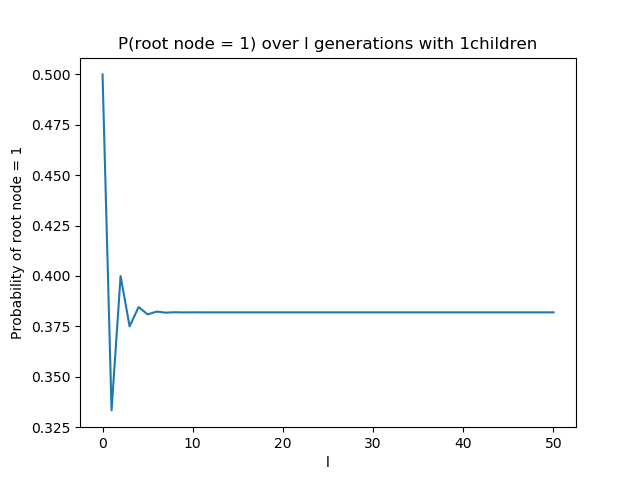
\includegraphics[width=0.5\textwidth]{p2_4_1.png}
	\caption{$P(RN=1)$ over $l = 0...50$ with 1 children}
\end{figure}
\begin{figure}[H]
	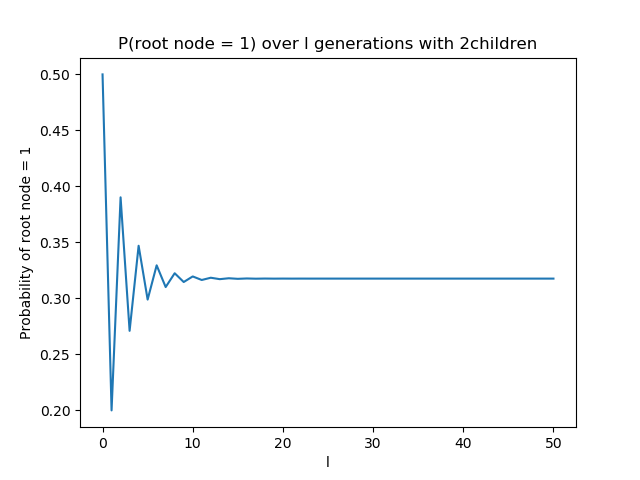
\includegraphics[width=0.5\textwidth]{p2_4_2.png}
	\caption{$P(RN=1)$ over $l = 0...50$ with 2 children}
\end{figure}
\begin{figure}[H]
	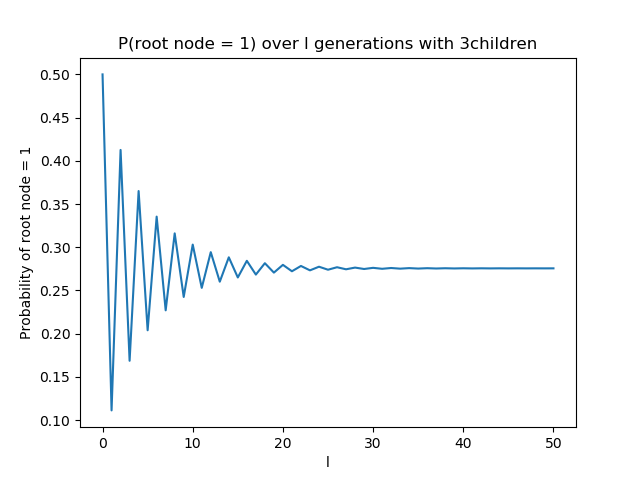
\includegraphics[width=0.5\textwidth]{p2_4_3.png}
	\caption{$P(RN=1)$ over $l = 0...50$ with 3 children}
\end{figure}
\begin{figure}[H]
	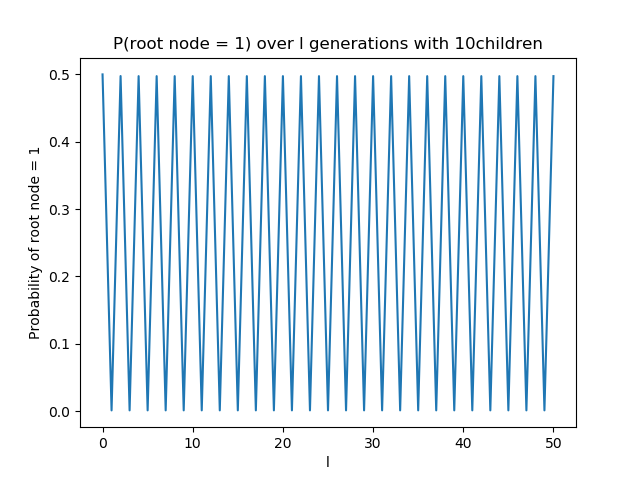
\includegraphics[width=0.5\textwidth]{p2_4_10.png}
	\caption{$P(RN=1)$ over $l = 0...50$ with 10 children: no convergence!}
\end{figure}
\subsection{d}
We can clearly see from the above that as our k increases, there seems to be a longer period (number of generations) necessary to achieve convergence, until there is some breaking point where convergence can not be achieved.
\\
\\ 
Using Banach's fixed point theorem, we can show that for $k\le 3$ our recursion established above converges over $l$, In this theorem, we will say that our $T(X)$ acts as our recursion, meaning $T(P_{l-1}) = P_l$ where $T(P_{l-1}) = (1-p_{l-1})^{-k} = p_l$. We want to show that for $k\le 3$ that $d(T(X),T(Y)) \le \phi d(X,Y)$ where d is a euclidean distance. Since our X and Y are scalars representing probabilities, this is just their Manhattan distance, or the absolute value of their difference. Further we need that our $\phi$ is upper bounded by one, so its fair to say $d(T(X),T(Y)) \le \d(X,Y)$ 
\\
There are 3 cases
\\
\\
Case 1: X=Y. which means that we have $X=Y=P_{l,k}(root = 1) \rightarrow 0 \le 0$ and we are done.
\\
\\
Case 2: $X<Y$. We want to show. $T(Y)-T(X) \le Y-X$. Thinking about this very intuitively, we can see that $(\frac{1}{1+p_{l}}) < 1$. When raised to the k, we still have it is less than one, lets call this $A$. When brought up in recursion, it means that the \textbf{previous} $p_{l+1}$ that drives from it $p_{l+1} = \frac{1}{1+A}$. We know that $p_l >0$ so then it must be true that out $p_{l+1} < 1$. However, as we can tell depending on how extreme our $k$ is, it will cause the previous one to that $p_{l+2}$ to fluctuate in the other direction. Consequently, if $k>3$, this will prove enough to no longer satisfy $T(Y)-T(X) \le Y-X \forall Y,X$ in the domain.
\\
\\
Case 3: $X>Y$. We want to show. $T(X)-T(Y) \le X-Y$. This is identical to the proof above just with some variables swapped around.

\section{3.1}

\subsection{a}
We have $A-(C\cup D)-B$ and $A-(B\cup D)-C \rightarrow \mu(X_A,X_B,X_C,X_D) = f(X_A,X_B,X_D)g(X_C,X_B,X_D) = a(X_A,X_C,X_D)b(X_C,X_B,X_D)$

\begin{gather}
\mu(X_A,X_B,X_C,X_D) = f(X_A,X_B,X_D)g(X_C,X_B,X_D) = a(X_A,X_C,X_D)b(X_C,X_B,X_D) \rightarrow \\
f(X_A,X_B,X_D) = \frac{a(X_A,X_C,X_D)b(X_C,X_B,X_D)}{g(X_C,X_B,X_D)} \rightarrow \\
f(X_A,X_B,X_D)= \frac{a(X_A,X_D)b(X_B,X_D)}{g(X_B,X_D)} \rightarrow \\
f(X_A,X_B,X_D) = a'(X_A,X_D)b'(X_B,X_D)   
\end{gather}
We can do the above because of the two conditional independencies we have assumed and the consequence afterwards of the equality between the two factorizations. Furthermore, it is easy to see that functions $b,g$ with the same variables space combined to form $b'$ and $a'=a$
\\


\subsection{b}
\begin{gather}
\mu(X_A,X_B,X_C,X_D) = f(X_A,X_B,X_D)g(X_C,X_B,X_D) \\
= a'(X_A,X_D)b'(X_B,X_D)g(X_C,X_B,X_D) \text{ from a} \\
\text{let } M(X_A,X_D) =  a'(X_A,X_D) \text{ and } N(X_B,X_C,X_D) = b'(X_B,X_D)g(X_C,X_B,X_D) \\
\rightarrow \mu(X_A,X_B,X_C,X_D)= M(X_A,X_D)N(X_B,X_C,X_D) \\
\end{gather}
Since $\mu(X_A,X_B,X_C,X_D)$ facotrizes in this way, we have shown that $A-D-(B\cup C)$

\subsection{c}
If $\mu$ were not strictly positive, then we would have some instances such that $\mu = 0$. Consider an instance where $\mu(1,1,1,1) = \mu(0,0,1,0) = \mu(0,0,1,1) = 1/3$ where our random variables $X_A,X_B,X_C,X_D$ are in that same order. The remaining space of 13 other join distributions are all zero. In this case, we can see that by know $X_C\cup X_D$ determines exactly what our $X_A$ and $X_B$ are entirely, so knowing anything about either $X_A$ or $X_B$ helps us better know what either random variable takes. The same goes for knowing $X_B\cup X_D$ determines exactly $X_A$ and $X_C$. However, we can clearly see that knowing $X_D$ is not deterministic for $X_A$ and $X_B\cup X_C$, as knowing $X_A$ helps us determine what values $X_B\cup X_C$ take. Thus this intersection lemma does not hold when we allow $\mu$ to take zero as a value

\begin{section}{Appendix}
	For question 2.2b, we have some additional steps here $(A-I\frac{1+\sqrt{5}}{2}) = $$\begin{bmatrix}
	\frac{1-\sqrt{5}}{2}&1 \\
	1&-\frac{1+\sqrt{5}}{2}
	\end{bmatrix}
	\begin{bmatrix}
	v_1 \\
	v_2
	\end{bmatrix} \rightarrow \frac{1-\sqrt{5}}{2}v_1 + v_2 = 0 $ and $v_1 -\frac{1-\sqrt{5}}{2}v_2 =0$  
	
	Solving for these gives us eigen vectors $\begin{bmatrix}
	1 \\
	\lambda_1
	\end{bmatrix}$,$\begin{bmatrix}
	1 \\
	\lambda_2
	\end{bmatrix}$
	The rest can be found and described here :
	https://www.math.wustl.edu/~freiwald/309fibonacci.pdf
	\\
	\\
	For question 3.1 c, this was an old response, logic was flawed, but was my initial mindset
	\\
	If $\mu$ were not strictly positive, then we would have some instances such that $\mu = 0$. This entire proof hangs on that we have $\frac{a(X_A,X_C,X_D)b(X_C,X_B,X_D)}{g(X_C,X_B,X_D)}$ well defined. And if there are some $\mu = 0$, we could imagine a case where $g(X_C,X_B,X_D) = 0$ which would render our results invalid. Thus we require that $\mu>0$ over its entire domain.
	\\
	\\
	This code used to generate plots and more will be posted on github soon @ user: bogyshi! stay posted!
	
\end{section}



\end{document}